\section{Funktionen}
	\todo[color=purple]{Kasten für Formel hinzufügen}
	\todo[color=purple]{Zusammenfassung-Kasten hinzufügen}
	\todo[color=purple]{Signalwörter-Kasten hinzufügen}
	Kommen wir kurz auf Funktionen im allgemeinen zu sprechen. Grundsätzlich werden
	Funktionen als f(x)=\ldots dargestellt (anstelle von f können wir den
	Funktionen natürlich auch andere Namen geben). Das x ist unsere Variable, das
	Ergebnis, dass wir dann bekommen, ist unser Wert an dieser Stelle. So ist für
	\(f(x)=x^2\) der Wert für die Stelle \(x=2:\ f(2)=2^2=4\).\\
	Doch was genau macht eine Funktion überhaupt? Sie weist jeder Zahl
	\underline{eine} andere Zahl zu. Letztendlich ist sogar ein Telefonbuch eine
	Funktion, denn sie weist jedem Namen eine Telefonnummer zu (jeder Name darf
	dann aber nur einmal vorkommen und nur eine Telefonnummer drin stehen haben,
	damit der Vergleich zulässig ist ;) ). Eine Funktion darf also zusätzlich keine
	Stelle mit zwei Werten haben. So darf also f(0)=1 und f(0)=3 nicht vorkommen!

	% Verschieben & strecken von Funktionen
	\subsection{Verschieben \& strecken von Funktionen}
\todo[color=red]{Kasten für Formel hinzufügen}
\todo[color=red]{Zusammenfassung-Kasten hinzufügen}
\todo[color=red]{Signalwörter-Kasten hinzufügen}
Bevor wir die Funktionsarten auflisten und beschreiben, wollen wir erst noch darauf eingehen, wie man Funktionen verschiebt und streckt. Für das bessere Verständnis zeigen wir das an den einzelnen Funktionen selbst noch einmal. Im Kommenden werden wir die ursprüngliche Funktion f(x) und die veränderten h(x) nennen.\\
\(\star\) Wollen wir eine Funktion nach oben oder unten verschieben, dann addieren wir einfach die entsprechende Zahl c hinzu (eine positive, um sie nach oben zu schieben und eine negative für selbiges nach unten), also \(h_1(x)=f(x)+c\).\\
\(\star\) Wollen wir die Funktion nach links oder rechts verschieben, so schreiben wir \(h_2(x)=f(x-b)\), wobei b die Verschiebung darstellt. \textit{Am Besten setzt ihr das (x-b) in Klammern} dort ein, wo zuvor das x war, so vermeidet ihr Fehler. Wollen wir sie nach rechts verschieben, so setzen wir für b eine positive Zahl ein (das - bleibt also), wollen wir sie nach links verschieben, so setzen wir für b entsprechend eine negative Zahl ein, wodurch ein + in der Klammer steht.\\
\(\star\) Kommen wir nun noch zur Streckung bzw. Stauchung. Haben wir eine Funktion und wollen sie strecken, so multiplizieren wir die Funktion einfach mit einer Zahl a>1. Die Stauchung erfolgt durch das multiplizieren mit 0<a<1, wodurch die Funktion an die x-Achse geschmiegt wird. Ist unser a negativ, dann wird unsere Funktion einfach an der x-Achse gespiegelt, die Streckung oder Stauchung bleibt aber, wie oben, von a abhängig. Dargestellt sieht das dann so aus: \(h_3(x)=a\cdot f(x)\).


	% Grundarten von Funktionen
	\subsection{Grundarten von Funktionen}
	\todo[color=purple]{Kasten für Formel hinzufügen}
	\todo[inline,color=red]{Zusammenfassung-Kasten hinzufügen}
	\todo[inline,color=red]{Signalwörter-Kasten hinzufügen}
	In den folgenden Seiten wollen wir euch die Grundfunktionen vorstellen, mit
	denen wir uns beschäftigen werden und letztlich auch ein paar Worte über
	zusammengesetzte Funktionen verlieren. Mit der Verschiebung und Zusammensetzung
	von Funktionen haben wir dann alle Funktionen betrachtet, welche ihr kennen
	sollt.

	\subsubsection{Lineare Funktionen \& deren Normale}
		\todo[color=green]{Kasten für Formel hinzufügen}
		\todo[inline,color=red]{Zusammenfassung-Kasten hinzufügen}
		\todo[inline,color=red]{Signalwörter-Kasten hinzufügen}
		Eine lineare Funktion stellt die leichteste Funktionenklasse dar. Als
		Schaubild haben wir eine Gerade. Dargestellt wird sie allgemein als:
		\formel{\[f(x)=m\cdot x+c\]}
		wobei c der y-Achsenabschnitt ist (dort schneidet sie diese) und m die
		Steigung (welche auch 0 sein darf)\footnote{Wir werden uns hier sparen, jede
		Funktion aufzuzeichnen. Das könnt ihr bequem mit dem Taschenrechner
		nachholen.}. Eine Normale bedeutet, dass sie im rechten Winkel zur
		eigentlichen Funktion steht. Das ist der Fall wenn folgendes gilt:
		\formel{\[m_2=-\frac{1}{m_1}\]}

	\subsubsection{Quadratische und andere ganzrationale Funktionen}
		\todo[color=green]{Kasten für Formel hinzufügen}
		\todo[inline,color=red]{Zusammenfassung-Kasten hinzufügen}
		\todo[inline,color=red]{Signalwörter-Kasten hinzufügen}
		\(\star\) Beschäftigen wir uns zunächst nur mit quadratischen Funktionen. Mit
		Verschiebungen wird aus \(x^2\):
		\formel{\[f(x)=a(x-b)^2+c\]}
		Der Faktor a gibt die Streckung an, was man unter Vorbehalt mit der Steigung
		der linearen Funktion vergleichen kann. Je größer der Faktor ist, desto
		schneller steigt die Funktion an. b  stellt die Verschiebung in x-Richtung dar
		und c ist die Verschiebung in y-Richtung.\\
		Wie man sehen kann, befindet sich in der Funktion eine binomische Formel,
		welche man ausklammern kann. Dann erhält man dieselbe Funktion anders
		geschrieben (wir haben hier noch die Faktoren umbenannt):
		\[f(x)=a_2 \cdot x^2+a_1 \cdot x+a_0\]

		\(\star\) Mit dieser Schreibweise kommen wir schon allgemein zu den
		ganzrationalen Funktionen:
		\formel{\[f(x)=a_n \cdot x^n+a_{n-1} \cdot x^{n-1}+\ldots +a_1 \cdot x+a_0\]}
		Wir haben also eine Funktion, bei der beliebig viele (positive und
		ganzzahlige) Potenzen von x, mit einem Faktor \(a_n\) (dieser darf auch
		negativ oder 0 sein) davor, summiert werden. Die höchste Potenz (hier n) nennt
		man den Grad der Funktion. Wieso das wichtig ist, werden wir später noch
		sehen, wenn wir das Verhalten von Funktionen im unendlichen betrachten. Eine
		Funktion mit dem Grad 1 ist eine lineare Funktion, eine mit dem Grad 0
		entspricht einer konstanten Funktion (eine lineare, mit der Steigung m=0).

	%Gebrochenrationale fliegen raus!	%\subsubsection{gebrochen rationale
	% Funktionen} Diese Funktionen sind 2 (meist unterschiedliche) ganzrationale
	% Funktionen, welche geteilt werden. Heißen unsere ganzrationalen Funktionen
	% f(x) und g(x), so ist unsere gebrochene rationale Funktion:
	%\[h(x)=\frac{f(x)}{g(x)}\]
	%Hier gilt nur zu beachten, dass es einen Grad im Nenner und einen im Zähler
	% gibt und dass sie im Gegensatz zu den ganzrationalen Funktionen eine
	% Definitionslücke haben können und zwar immer dann, wenn im Nenner 0 heraus
	% kommt (vergleiche \(\frac{1}{x}\)).

	\subsubsection{Exponentiale Funktionen}
		\todo[color=green]{Kasten für Formel hinzufügen}
		\todo[inline,color=red]{Zusammenfassung-Kasten hinzufügen}
		\todo[inline,color=red]{Signalwörter-Kasten hinzufügen}
		%\& logarithmische Funktionen
		Diese hatten wir ja vorhin schon einmal angesprochen. Ein Beispiel für eine
		Exponentialfunktion (mit der Basis 2) ist \(2^x\). Allerdings ist 2 eine
		ungeschickte Basis beim Ableiten. Unter anderem deswegen nutzt man als Basis
		die eulersche Zahl e=2,71828\ldots \ . Im Pflichtteil braucht ihr den
		Logarithmus oder das Exponential von e nicht ausrechnen (es sei denn, es ist
		trivial) und könnt sie einfach so hinschreiben (z. B. \(e^3\)). Genau so geht
		das übrigens bei allen irrationalen Zahlen wie z. B. \(\pi\).\\
		Umrechnen in eine e-Funktion lässt sich unser Beispiel leicht. Da der ln die
		Umkehrfunktion der e-Funktion ist gilt: \(f(x)=2^x=e^{ln(2)\cdot x}\).
		Grundsätzlich stellen wir e-Funktionen so dar:
		\formel{\[f(x)=a \cdot e^{b(x-c)}+d\]}
		a ist wieder die Streckung, ähnlich wie bei den quadratischen Funktionen. Das
		b ist auch eine Art Streckung (sie entspricht dem ln, wenn wir eine Funktion
		umschreiben). c verschiebt wieder in x-Richtung und d in y-Richtung.\\
		%Nun noch zu den Logarithmusfunktionen. Wie schon erwähnt, sind diese die
		% Umkehrfunktionen der e-Funktion\footnote{Was genau das heißt, sieht man
		% gerade bei den beiden Funktionen sehr schön, wenn man beide Zeichnen
		% lässt.
		% Abstrakter kann man sich das so klar machen: Haben wir die e-Funktion, so
		% vertauschen wir x und y einfach und lösen wieder nach y=\ldots auf.}.
		% Darstellen lassen sie sich als: \[f(x)=a\cdot ln(b(x-c))+d\] a ist wieder
		% die Streckung, c und d die Verschiebung und b ist ähnlich geartet wie das b
		% bei den e-Funktionen.

	\subsubsection{Trigonometrische Funktionen}
		\todo[color=purple]{Kasten für Formel hinzufügen}
		\todo[inline,color=red]{Zusammenfassung-Kasten hinzufügen}
		\todo[inline,color=red]{Signalwörter-Kasten hinzufügen}
		Die trigonometrischen Funktionen bilden einen wichtigen Teil in der Analysis.
		Mit ihnen werden sich wiederholende Vorgänge beschrieben. Auch sind die
		Ableitungen und Integrale, ähnlich wie bei den e-Funktionen, sehr einfach.
		Dafür erfordert es ein größeres Maß an Konzentration, um die Grunddefinitionen
		zu verstehen. Deshalb werden wir dieses Thema ausführlich in 3 Unterkapiteln
		erklären.
		\paragraph{Bogenmaß}
			\todo[color=green]{Kasten für Formel hinzufügen}
			\todo[inline,color=red]{Zusammenfassung-Kasten hinzufügen}
			\todo[inline,color=red]{Signalwörter-Kasten hinzufügen}
			Das Bogenmaß ist in mathematischer Sicht eingänglicher und wird deshalb auch
			öfter benutzt als Gradzahlen. Beide beschreiben jedoch einen Winkel.
			Definiert ist das Bogenmaß über den Umfang des Einheitskreises. Schauen wir
			uns einmal den Einheitskreis an.\\
			Dieser hat den Radius 1 (daher Einheitskreis). Der Umfang des kompletten
			Kreises beträgt \(2\pi\). Diese Entsprechen den \(360^\circ\). Haben wir eine
			\(180^\circ\) Wende, so entspricht das dem Umfang eines halben
			Einheitskreises im Bogenmaß, also \(\pi\) \footnote{Beide Angaben geben das
			gleiche an, allerdings in unterschiedlichen Einheiten. Mit der Umrechnung
			verhält es sich ähnlich wie mit Yards und Metern.}. Allgemein gilt immer das
			Verhältnis \(\frac{\beta}{2\pi}=\frac{\alpha}{360^\circ}\), wobei \(\alpha\)
			unser Winkel in Grad ist und \(\beta\) der Winkel in Bogenmaß. Als
			Umrechnungsformel könnt ihr Folgendes benutzen :
			\formel{\[\beta=\frac{\pi \cdot \alpha}{180^\circ}\]}
			\underline{\textbf{VORSICHT:}} Achtet immer darauf, dass euer Taschenrechner
			richtig eingestellt ist! Rechnet ihr mit Bogenmaß, so sollte im
			Taschenrechner an entsprechender Stelle "Bog" stehen. Rechnet ihr mit Grad,
			so an gleicher Stelle "Gra" !!!
		\paragraph{Definition am Einheitskreis}
			\todo[color=green]{Kasten für Formel hinzufügen}
			\todo[inline,color=red]{Zusammenfassung-Kasten hinzufügen}
			\todo[inline,color=red]{Signalwörter-Kasten hinzufügen}
	   
			\begin{figure}[h]
				\centering
				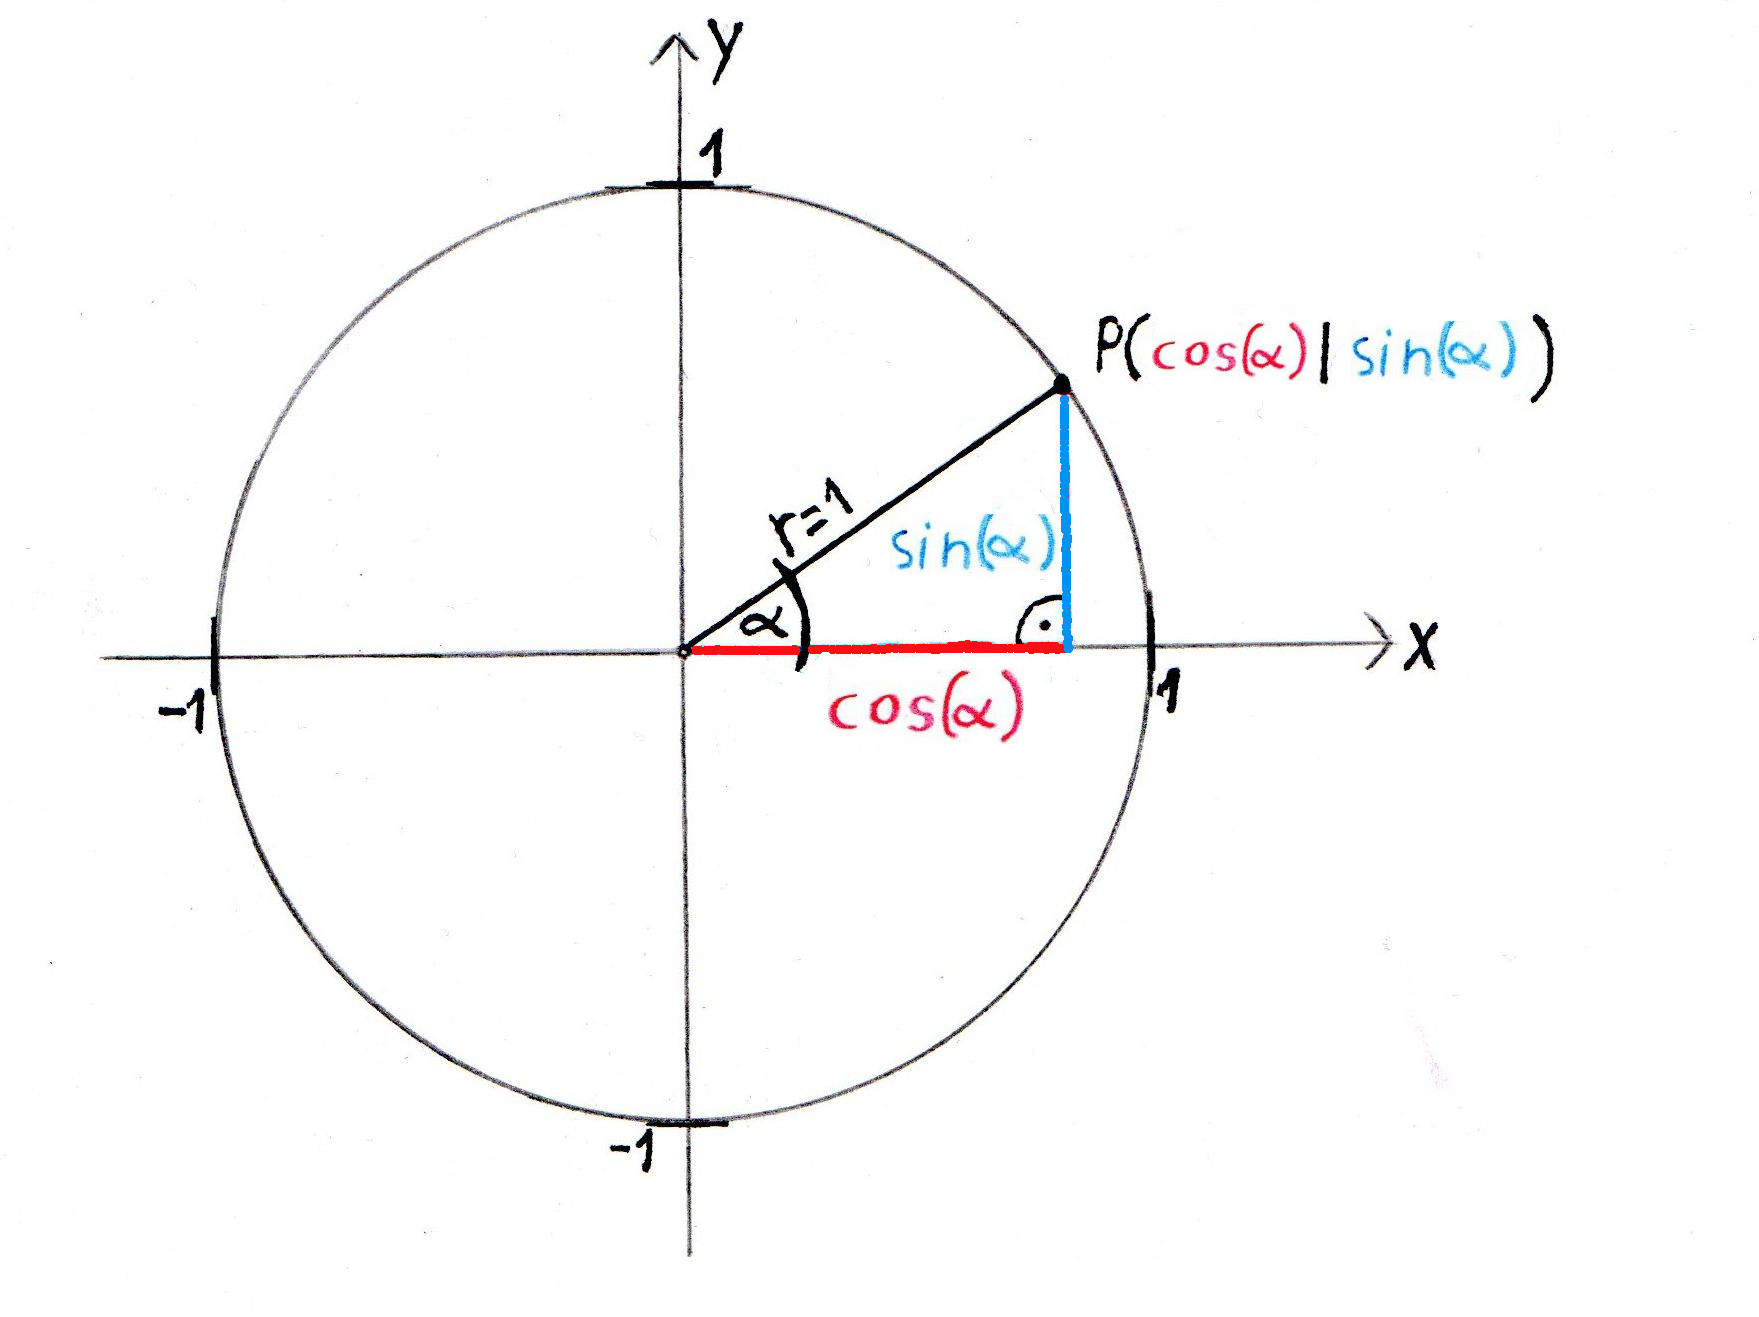
\includegraphics[scale=0.2]{Images/Einheitskreis.jpeg}
				\caption{Sinus \& Kosinus am Einheitskreis}
			\end{figure}
  
			Das Bild soll uns die Definition der trigonometrischen Funktionen erklären.
			Der Radius des Kreises ist 1. Somit wird die schräge Linie dies auch immer
			sein, egal in welchem Winkel \(\alpha\) sie zur x-Achse steht. Letzterer ist
			beliebig wählbar. Die rote Linie ist nun der Kosinus in Abhängigkeit des
			Winkels und die blaue Linie entspricht dem Sinus. Ist der Winkel 0, so ist
			unser Sinus (der y-Wert, an der die Gerade den Kreis schneidet) ebenfalls 0,
			der Kosinus (der x-Wert) entsprechend 1. Hier wird vielleicht auch
			ersichtlich, wieso sich das ganze wiederholt. Wenn nicht, empfehlen wir euch
			folgendem Link nachzugehen und durch ein wenig Ausprobieren die Funktion
			besser kennen zu lernen. Ein Dankeschön an dieser Stelle an den Autor des
			Applets Walter Fendt, welcher uns erlaubt, seine Applets zu nutzen ):
			\url{http://www.walter-fendt.de/m14d/sincostan.htm}\\
			Zuletzt noch der Tangens. Wie der Wert am Einheitskreis festgelegt ist (auch
			im Link) spielt keine große Rolle. Definiert ist er einfach als
			\(tan(x)=\frac{sin(x)}{cos(x)}\).\\
			Wir möchten noch kurz ansprechen, wie wir die trigonometrischen Funktionen in
			der Mittelstufe benutzt haben. Damit könnt ihr zum Beispiel den Winkel
			zwischen einer Funktion (bzw. deren Steigung an dem Punkt) und der x-Achse
			bestimmen. So ist bei einem rechtwinkligen Dreieck die längste Seite
			(gegenüber vom rechten Winkel) die Hypotenuse (kurz h), die Seite am Winkel
			\(\alpha\) nennt man die Ankathete (kurz a) und die andere, gegenüber des
			Winkels ist die Gegenkathete (kurz g). Damit gilt dann:
			\formel{\[sin(\alpha)=\frac{g}{h},\ cos(\alpha)=\frac{a}{h},\
			tan(\alpha)=\frac{g}{a}\]}
		\paragraph{sin, cos \& tan als Funktion}
			\todo[color=green]{Kasten für Formel hinzufügen}
			\todo[inline,color=red]{Zusammenfassung-Kasten hinzufügen}
			\todo[inline,color=red]{Signalwörter-Kasten hinzufügen}
			Wie wir schon zuvor angekündigt hatten, ist bei diesen Funktionen viel zu
			beachten. Wir möchten als Beispiel den Sinus nutzen, um euch das Prinzip zu
			erklären. Der Kosinus funktioniert aber genau so (er ist nur verschoben, wie
			wir später sehen werden). Den Tangens werden wir nur kurz andeuten, da er
			nicht oft vorkommt.\\
			Grundsätzlich stellen wir den Sinus so dar:
			\formel{\[f(x)=a\cdot sin(b(x-c))+d\]}	
			Betrachten wir zuerst die bekannten und daher einfachen Konstanten. c
			verschiebt wieder nach links oder rechts und das d nach oben oder unten.
			Verschiebt man den Kosinus um \(\frac{\pi}{2}\) nach rechts, so erhält man
			den Sinus, verschiebt man ihn um die gleiche Länge nach links, hat man den
			-sin(x) (genauer um eine \(\frac{1}{4}\) Periode, wenn diese nicht \(2 \pi\)
			ist):
			\[sin(x)=cos(x-\frac{\pi}{2})\ \&\ cos(x)=sin(x+\frac{\pi}{2})\]
			 Das a ist letztendlich wieder eine Streckung. Hier fällt einem jedoch
			 zusätzlich etwas auf: Ist das a nicht da, (wir nehmen jetzt mal an, dass die
			 Funktion nicht verschoben wurde) so haben alle Hochpunkte den Wert 1 und
			 alle Tiefpunkte den Wert -1. Mit a sind alle Werte zwischen a und -a.
			 Selbiges bei einem verschobenen Graphen herauszufinden, ist etwas komplexer.
			 Wir nehmen einfach den höchsten Punkt und ziehen ihn vom niedrigsten ab und
			 teilen durch 2. Ein kleines Beispiel: Haben die Hochpunkte den Wert y=4 und
			 die Tiefpunkte den Wert y=0, so rechnen wir \(a=\frac{4-0}{2}=2\).\\
 			Nun kommen wir noch zum b. Hierzu müssen wir erst einmal wissen, was eine
 			Periode ist. Diese gibt an, wie lange es dauert, bis die Funktion wieder am
			 gleichen Status ist, wie zuvor auch schon (sie wiederholt sich ja
			 periodisch).
			 Am besten schaut man, wie der Abstand von Hochpunkt zu Hochpunkt ist. Bei
			 b=1 wären das \(2\pi\) also gerade eine Umdrehung im Einheitskreis. Durch
			 das b verändert sich aber die Periode p und zwar nach folgender Gleichung:
 			\formel{\[p=\frac{2\pi}{b}\]}
			 Die Erkenntnisse für den Sinus (und somit auch für den Kosinus) gelten auch
 			für den Tangens, mit folgender Ausnahme: Beim Tangens gibt es keine
 			Amplitude, die Streckung erfolgt also wie bei den vorherigen Funktionen.\\
 			Auch wenn wir uns hier wiederholen, aber schaut bitte unbedingt, dass euer
 			Taschenrechner mit der richtigen Winkeleinheit rechnet! Bei den
 			\textit{trigonometrischen Funktionen} nehmt am besten immer das Bogenmaß,
 			abgesehen davon, dass es sowieso meistens gebraucht wird, sehen eure Kurven
 			auf dem Taschenrechner sonst eigenartig aus und ihr lauft Gefahr, dass die
 			Rechnungen falsch sind.

%Wurzelfunktionen fliegen raus 
% \subsubsection{Wurzelfunktionen}
%Eine letzte Funktionenklasse stellt die Wurzelfunktion dar. Allgemein hat sie folgende Form:
%\[f(x)=a\sqrt[n]{b(x-c)}+d\]
%c und d Verschieben wieder, a streckt die Funktion und das b ist wieder ähnlich dem der e-Funktion (streckt also wieder in gewisser Art).


	% Zusammengesetzte Funktionen
	\section{Zusammengesetzte Funktionen}
	\todo[color=purple]{Kasten für Formel hinzufügen}
	\todo[color=purple]{Zusammenfassung-Kasten hinzufügen}
	\todo[color=purple]{Signalwörter-Kasten hinzufügen}
	Unsere Grundfunktionen können wir nun beliebig kombinieren (im Folgenden sind
	die Grundfunktionen immer als f(x) und g(x) dargestellt, die Resultierende
	nennen wir h(x)). Dieses Kapitel dient zum einen dem tieferen Verständnis der
	Materie, aber vor allem wird es uns helfen, die Ableitungs-/ \& Integral-Regeln
	zu verstehen und richtig anwenden zu können\footnote{Natürlich lassen die drei
	Möglichkeiten sich auch noch einmal miteinander kombinieren. Das werden wir im
	Kurs an einigen Beispielen sehen.}. Wenn ihr zwei Funktionen kombiniert, so
	setzt einfach die Funktion für das entsprechende f(x) oder g(x) ein.

	\subsection{Summe \& Differenzen}
		\todo[color=green]{Kasten für Formel hinzufügen}
		\todo[color=purple]{Zusammenfassung-Kasten hinzufügen}
		\todo[color=green]{Signalwörter-Kasten hinzufügen}
		Die einfachste Form ist das Addieren und Subtrahieren von zwei Funktionen.
		Dies wird vor allem nötig sein im Wahlteil, wenn man z. B. die Fläche
		berechnen will, die von zwei Funktionen eingeschlossen wird (zuerst ziehen wir
		die Funktionen voneinander ab und integrieren dann). Die Darstellung sieht
		folgendermaßen aus:
		\formel{\[h_1(x)=f(x)+g(x), \mathrm{\ bzw\ } h_2(x)=f(x)-g(x)\]}
		
		\tags{
			Summenregel
		}
	
	\subsection{Produkte \& Quotienten}
		\todo[color=green]{Kasten für Formel hinzufügen}
		\todo[color=purple]{Zusammenfassung-Kasten hinzufügen}
		\todo[color=green]{Signalwörter-Kasten hinzufügen}
		Diese Regel bei einer Funktion zu erkennen, wird uns helfen, die Faktorregel
		beim Ableiten und Integrieren anwenden zu können:
		\formel{\[h_1(x)=f(x)\cdot g(x), \mathrm{\ bzw\ } h_2(x)=\frac{f(x)}{g(x)}\]}
		
		\tags{
			Produktregel
		}

	\subsection{Verkettungen}
		\todo[color=green]{Kasten für Formel hinzufügen}
		\todo[color=purple]{Zusammenfassung-Kasten hinzufügen}
		\todo[color=green]{Signalwörter-Kasten hinzufügen}
		Eine letzte Kombination stellt die Verkettung dar. Diese werden wir beim
		Ableiten bei der Kettenregel wieder erkennen. Allgemein beschreibt man das so:
		\formel{\[h(x)=f(g(x))\]}
		Wir ersetzen also bei f(x) jedes x durch die Funktion in g(x) (alles in
		Klammern schreiben). Ein kleines Beispiel für das Verständnis: mit \(f(x)=e^x\
		\&\ g(x)=2x+3\) gilt \(h(x)=f(g(x))=e^{2x+3}\).
		
		\tags{
			Kettenregel
		}

